%
% overall.tex
%
% Copyright (C) 2021 by SpaceLab.
%
% FloripaSat-2 Documentation
%
% This work is licensed under the Creative Commons Attribution-ShareAlike 4.0
% International License. To view a copy of this license,
% visit http://creativecommons.org/licenses/by-sa/4.0/.
%

%
% \brief Overall description chapter.
%
% \author Gabriel Mariano Marcelino <gabriel.mm8@gmail.com>
%
% \institution Universidade Federal de Santa Catarina (UFSC)
%
% \version 0.1.0
%
% \date 2020/06/05
%

\chapter{Overall Description} \label{ch:overall}

.

\section{General Diagrams}

The CubeSat's subsystems are positioned in the 2U physical structure as exemplified in \autoref{fig:subsystems-positioning}. An exploded 3D view of the satellite is showed in \autoref{fig:exploded-view}.

\begin{figure}[!ht]
    \begin{center}
        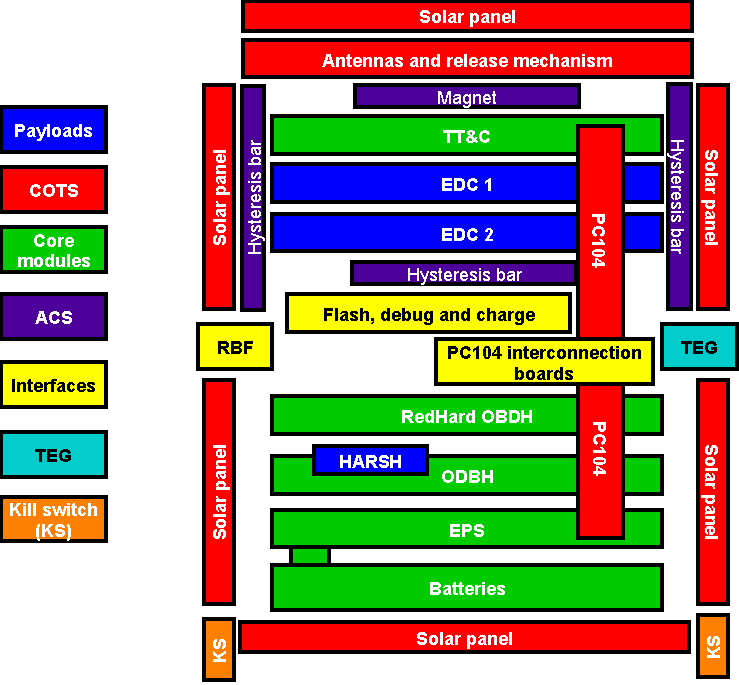
\includegraphics[width=0.7\textwidth]{figures/subsystems-positioning.pdf}
        \caption{Subsystems positioning.}
        \label{fig:subsystems-positioning}
    \end{center}
\end{figure}

%   TBD 
%   In \autoref{fig:datapath-diagram} there is a block diagram showing the satellite modules and the internal communication interfaces.

\section{General Behaviour}

.

\section{Orbit Parameters}

.

\section{Power Budget}

.

\section{Link Budget}

The link budget of all radio links of the satellite is available in \autoref{tab:link-budget-results}.

\begin{table}[!h]
    \centering
    \begin{tabular}{L{0.3\textwidth}ccccc}
        \toprule[1.5pt]
        \textbf{Variable} & \textbf{Beacon} & \textbf{Downlink} & \textbf{Uplink} & \textbf{Uplink (Payload)} & \textbf{Unit}\\
        \midrule
        Frequency                       & 145,97    & 436,9     & 436,9     & 401,635   & MHz \\
        Modulation                      & GMSK      & GMSK      & GMSK      & BPSK      & - \\
        Protocol                        & NGHam     & NGHam     & NGHam     & SBCD      & - \\
        Transmit power                  & 30        & 30        & 47        & ??        & dBm \\
        FSPL                            & 144,8     & 154,3     & 154,3     & ??        & dB \\
        Other losses                    & 5         & 5         & 7         & 5         & dB \\
        Receive antenna gain            & 12        & 15.5      & 0         & 0         & dBi \\
        Receiver noise temp.            &           &           &           &           & K \\
        Antenna noise temp.             &           &           &           &           & K \\
        System noise temp.              &           &           &           &           & K \\
        Data rate                       & 1200      & 4800      & 4800      & 400       & bps \\
        Received SNR                    & 30,87     & 17,35     & 31,60     & ??        & dB \\
        SNR required for $10^{-5}$ BER*  & 9,6       & 9,6       & 9,6       & 9,6       & dB \\
        Link margin                     & $\leq$ 21,27 & $\leq$ 7,75 & $\leq$ 22 & $\leq$ ?? & dB \\
        \bottomrule[1.5pt]
    \end{tabular}
    \caption{Link budget results.}
    \label{tab:link-budget-results}
\end{table}

All equations and steps used to obtain the results of \autoref{tab:link-budget-results} are available in \autoref{anx:link-budget}.

\section{PC-104 Bus}

\begin{figure}[!ht]
    \begin{center}
        \includegraphics[width=0.5\textwidth]{figures/pc104-diagram}
        \label{fig:pc104-diagram}
        \caption{Reference diagram of the PC-104 bus.}
    \end{center}
\end{figure}

\begin{table}[!h]
    \centering
    \begin{tabular}{cllll}
        \toprule[1.5pt]
        \textbf{Pin Row}   & \textbf{H1 Odd}  & \textbf{H1 Even} & \textbf{H2 Odd} & \textbf{H2 Even} \\
        \midrule
        1-2                & -                & -                & -               & -                \\
        3-4                & -                & -                & EDC\_1\_EN      & EDC\_2\_EN       \\
        5-6                & -                & -                & BE\_UART\_RX    & -                \\
        7-8                & RA\_GPIO\_0      & RA\_GPIO\_1      & BE\_UART\_TX    & GPIO\_0          \\
        9-10               & RA\_GPIO\_2      & BE\_EN           & -               & -                \\
        11-12              & RA\_RESET        & RA\_EN           & BE\_SPI\_MOSI   & BE\_SPI\_CLK     \\
        13-14              & -                & -                & BE\_SPI\_CS     & BE\_SPI\_MISO    \\
        15-16              & -                & -                & -               & -                \\
        17-18              & EDC\_UART\_RX/TX & PLX\_EN          & -               & GPIO\_1          \\
        19-20              & EDC\_UART\_TX/RX & GPIO\_2          & -               & GPIO\_3          \\
        21-22              & -                & -                & -               & GPIO\_4          \\
        23-24              & -                & -                & -               & -                \\
        25-26              & -                & -                & PL\_VCC         & PL\_VCC          \\
        27-28              & -                & -                & TTC\_VCC        & TTC\_VCC         \\
        29-30              & GND              & GND              & GND             & GND              \\
        31-32              & GND              & GND              & GND             & GND              \\
        33-34              & -                & -                & -               & -                \\
        35-36              & RA\_SPI\_CLK     & -                & ANT\_VCC        & ANT\_VCC         \\
        37-38              & RA\_SPI\_MISO    & -                & -               & -                \\
        39-40              & RA\_SPI\_MOSI    & RA\_SPI\_CS      & -               & -                \\
        41-42              & PL\_I2C\_SDA     & -                & -               & GPIO\_5          \\
        43-44              & PL\_I2C\_SCL     & -                & -               & -                \\
        45-46              & OBDH\_VCC        & OBDH\_VCC        & BAT\_VCC        & BAT\_VCC         \\
        47-48              & PL\_VCC          & PL\_VCC          & -               & -                \\
        49-50              & RA\_VCC          & RA\_VCC          & EPS\_I2C\_SDA   & -                \\
        51-52              & BE\_VCC          & BE\_VCC          & EPS\_I2C\_SCL   & -                \\
        \bottomrule[1.5pt]
    \end{tabular}
    \caption{PC-104 bus pinout.}
    \label{tab:pc104-pinout}
\end{table}

\begin{table}[!h]
    \centering
    \begin{tabular}{lL{0.18\textwidth}L{0.17\textwidth}L{0.33\textwidth}}
        \toprule[1.5pt]
        \textbf{Signal}  & \textbf{Pin(s)} & \textbf{Used By}     & \textbf{Description} \\
        \midrule
        GND              & H1-29/30/31/32, H2-29/30/31/32 & All   & Ground reference \\
        BAT\_VCC         & H2-45, H2-46    & EPS                  & Battery terminals (+) \\
        ANT\_VCC         & H2-35, H2-36    & EPS, ANT             & Antenna power supply (3.3 V) \\
        OBDH\_VCC        & H1-45, H1-46    & EPS, OBDH            & OBDH power supply (3.3 V) \\
        TTC\_VCC         & H2-27, H2-28    & EPS, TTC             & TTC power supply (3.3 V) \\
        PL\_VCC          & H1-47/48, H2-25/26 & EPS, EDC 1/2, Payload X & Payloads power supply (5 V) \\
        RA\_VCC          & H1-49, H1-50    & EPS, TTC             & Main radio power supply (5 V) \\
        BE\_VCC          & H1-51, H1-52    & EPS, TTC             & Beacon power supply (6 V) \\
        RA\_SPI\_CLK     & H1-35           & OBDH, TTC            & CLK signal of the main radio SPI bus \\
        RA\_SPI\_MISO    & H1-37           & OBDH, TTC            & MISO signal of the main radio SPI bus \\
        RA\_SPI\_MOSI    & H1-39           & OBDH, TTC            & MOS signal of the main radio SPI bus \\
        RA\_SPI\_CS      & H1-40           & OBDH, TTC            & CS signal of the main radio SPI bus \\
        EPS\_I2C\_SDA    & H2-49           & OBDH, EPS            & SDA signal of the EPS I2C bus \\
        EPS\_I2C\_SCL    & H2-51           & OBDH, EPS            & SCL signal of the EPS I2C bus \\
        BE\_UART\_RX     & H2-5            & EPS, TTC             & EPS TX, Beacon RX (UART bus) \\
        BE\_UART\_TX     & H2-7            & EPS, TTC             & EPS RX, Beacon TX (UART bus) \\
        EDC\_UART\_TX/RX & H1-25           & OBDH, EDC 1/2        & OBDH TX, EDCs RX (UART bus) \\
        EDC\_UART\_RX/TX & H1-27           & OBDH, EDC 1/2        & OBDH RX, EDCs TX (UART bus) \\
        BE\_EN           & H1-10           & EPS, TTC             & Beacon radio power enable \\
        RA\_EN           & H1-12           & EPS, OBDH            & Main radio power enable \\
        EDC\_1\_EN       & H2-3            & OBDH, EDC 1          & EDC 1 enable signal \\
        EDC\_2\_EN       & H2-4            & OBDH, EDC 2          & EDC 2 enable signal \\
        PLX\_EN          & H1-18           & OBDH, Payload X      & Payload X enable (GPIO) \\
        PL\_I2C\_SDA     & H1-41           & OBDH, Payload X      & SDA signal of the payload I2C bus \\
        PL\_I2C\_SCL     & H1-43           & OBDH, Payload X      & SCL signal of the payload I2C bus \\
        GPIO\_N          & H1-20, H2-8/18/20/22/42  & OBDH        & GPIO pin (not used) \\
        \bottomrule[1.5pt]
    \end{tabular}
    \caption{PC-104 bus signal description.}
    \label{tab:pc104-signals}
\end{table}

\section{Telecommunication}

\begin{landscape}
    \begin{table}[ht]
        \centering
        \begin{tabular}{llccccc}
            \toprule[1.5pt]
            \multirow{2}{*}{\textit{Link}} & \multirow{2}{*}{\textit{Packet Name}} & \multicolumn{4}{c}{\textit{Payload}} & \multirow{2}{*}{\textit{Access}} \\
            \cmidrule{3-6}
                                      &                       & \textit{ID}  & \textit{Source Callsign}   & \textit{Data (up to 220 bytes)}            & \textit{Size (bytes)} & \\
            \midrule
            \multirow{2}{*}{Beacon}   & EPS data              & 00h & \multirow{2}{*}{``0'' + ``PY0EGU''} & EPS data                                   & 58                    & Public \\
                                      & TTC Data              & 01h &                                     & TTC data                                   & 18                    & Public \\
            \midrule
            \multirow{8}{*}{Downlink} & Telemetry             & 20h & \multirow{8}{*}{``0'' + ``PY0EGU''} & Flags + OBDH/EPS data                      & 220                   & Public \\
                                      & Ping answer           & 21h &                                     & Requester callsign                         & 15                    & Public \\
                                      & Data request answer   & 22h &                                     & Req. callsign + data                       & 15 to 155             & Public \\
                                      & Message broadcast     & 23h &                                     & Req. + dst. callsign + message             & 22 to 60              & Public \\
                                      & Hibernation feedback  & 24h &                                     & Req. callsign + hibernation in hours       & 17                    & Public \\
                                      & EDC info              & 25h &                                     & PTT decoder + HK info + system state       & 79                    & Public \\
                                      & EDC samples           & 26h &                                     & Timestamp + pkt. counter + samples         & 219                   & Public \\
                                      & TC feedback           & 27h &                                     & Req. callsign + TC packet ID + timestamp   & 13                    & Public \\
            \midrule
            \multirow{14}{*}{Uplink}  & Ping Request          & 40h & \multirow{14}{*}{Any Callsign}      & None                                       & 8                     & Public \\
                                      & Data Request          & 41h &                                     & Data flags + count + origin + offset       & 16                    & Public \\
                                      & Broadcast Message     & 42h &                                     & Dst. callsign + message                    & 15 to 46              & Public \\
                                      & Enter hibernation     & 43h &                                     & Req. callsign + hibernation in hours + key & 29                    & Private \\
                                      & Leave hibernation     & 44h &                                     & Command key                                & 16                    & Private \\
                                      & Activate beacon       & 45h &                                     & Command key                                & 16                    & Private \\
                                      & Deactivate beacon     & 46h &                                     & Command key                                & 16                    & Private \\
                                      & Activate downlink     & 47h &                                     & Command key                                & 16                    & Private \\
                                      & Deactivate downlink   & 48h &                                     & Command key                                & 16                    & Private \\
                                      & Activate EDC          & 49h &                                     & Command key                                & 16                    & Private \\
                                      & Deactivate EDC        & 4Ah &                                     & Command key                                & 16                    & Private \\
                                      & Activate Payload X    & 4Bh &                                     & Command key                                & 16                    & Private \\
                                      & Deactivate Payload X  & 4Ch &                                     & Command key                                & 16                    & Private \\
                                      & Get EDC info          & 4Dh &                                     & Command key                                & 16                    & Private \\
            \bottomrule[1.5pt]
        \end{tabular}
        \caption{Telecommunication packets and their content.}
        \label{tab:packets-struct}
    \end{table}
\end{landscape}
